\documentclass[aspectratio=43, a4paper, 12pt]{beamer}

% Packages
\usepackage{animate}
\usepackage{graphicx}
\usepackage{multicol}
\usepackage{charter}

% Language
\usepackage[utf8]{inputenc}
\usepackage[T1]{fontenc}
\usepackage{babel}


% Beamer
\usetheme{Singapore}
\usecolortheme{default}

\setbeamertemplate{items}[ball]
\setbeamertemplate{section in toc}[ball]
\setbeamertemplate{subsection in toc}[ball]
\setbeamercolor{section number projected}{bg=gray,fg=white}
\setbeamercolor{subsection number projected}{bg=gray, fg=white}
\setbeamercolor{item}{fg=gray}
\setbeamercolor{navigation symbols}{fg=black}
\addtobeamertemplate{background canvas}{\transfade[duration=0.2]}{}

\setbeamertemplate{navigation symbols}{}

\AtBeginSection[]
{
  \begin{frame}<beamer>
    \tableofcontents[currentsection]
  \end{frame}
}


% Footline
\definecolor{author_bg}{RGB}{204, 204, 236}
\setbeamercolor*{author_foot}{bg=author_bg, fg=black}
\setbeamercolor*{title_foot}{parent=palette secondary}

\setbeamertemplate{footline}
{	
	\hbox{
	 	\begin{beamercolorbox}[wd=0.5\paperwidth, ht=2.25ex, dp=1ex, right]{title_foot}
			\insertshorttitle \hspace{1em} 
		\end{beamercolorbox}%
		
	 	\begin{beamercolorbox}[wd=0.4\paperwidth, ht=2.25ex, dp=1ex, left]{author_foot}
		   	\hspace{1em} \insertshortauthor
	  	\end{beamercolorbox}%
	  	
	  	\begin{beamercolorbox}[wd=0.1\paperwidth, ht=2.25ex, dp=1ex, left]{author_foot}
		   	\hspace{1em} \insertframenumber~|\ \inserttotalframenumber
	  	\end{beamercolorbox}%	  	 
	}
}


\title{Modèle de \textsc{Vicsek}}
\subtitle{Soutenance finale de projet numérique}
\author{Antoine \textsc{Royer} \& Alexis \textsc{Peyroutet}}
\institute{L3 PCAME – Tarbes}
\date{}

\begin{document}
	\begin{frame}
		\titlepage
		
\includegraphics[width=3cm]{images/ut3.png} \hfill 
\includegraphics[width=2.5cm]{images/uppa.png}
	\end{frame}
	
\section{Présentation et explication}
\subsection{Présentation du modèle}
\begin{frame}{Présentation du modèle}
		\begin{columns}
			\begin{column}{0.5\paperwidth}
			\only<1>{\begin{center} 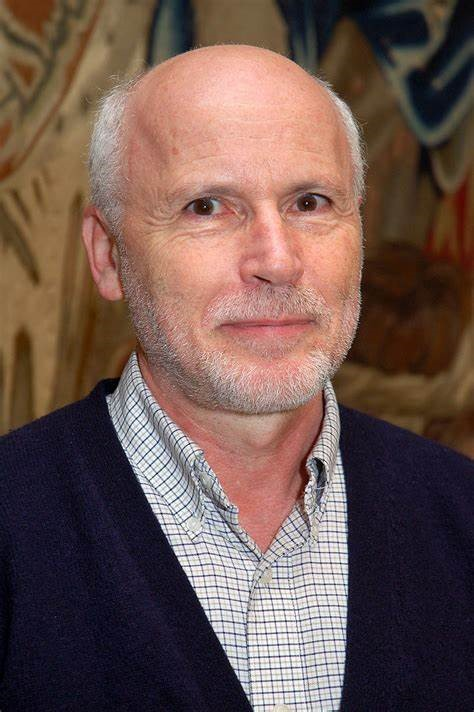
\includegraphics[width=4cm]{images/photo_vicsek.jpg}  \end{center}}
			\only<2>{\begin{center} 
\includegraphics[width=6cm]{images/calendrier.jpg} \end{center}}
			\only<3>{\begin{center} 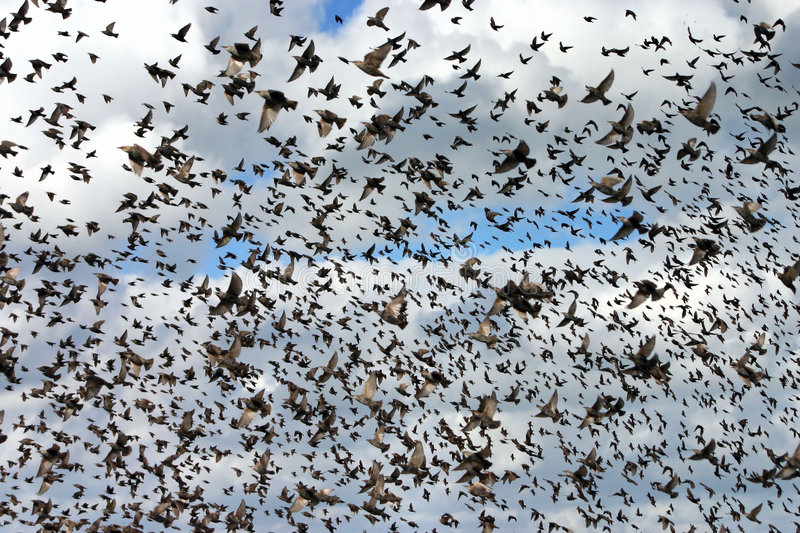
\includegraphics[width=6cm]{images/essaim_oiseau.jpg} \\ Essaim d'oiseaux \end{center}}
			\only<4>{\begin{center} 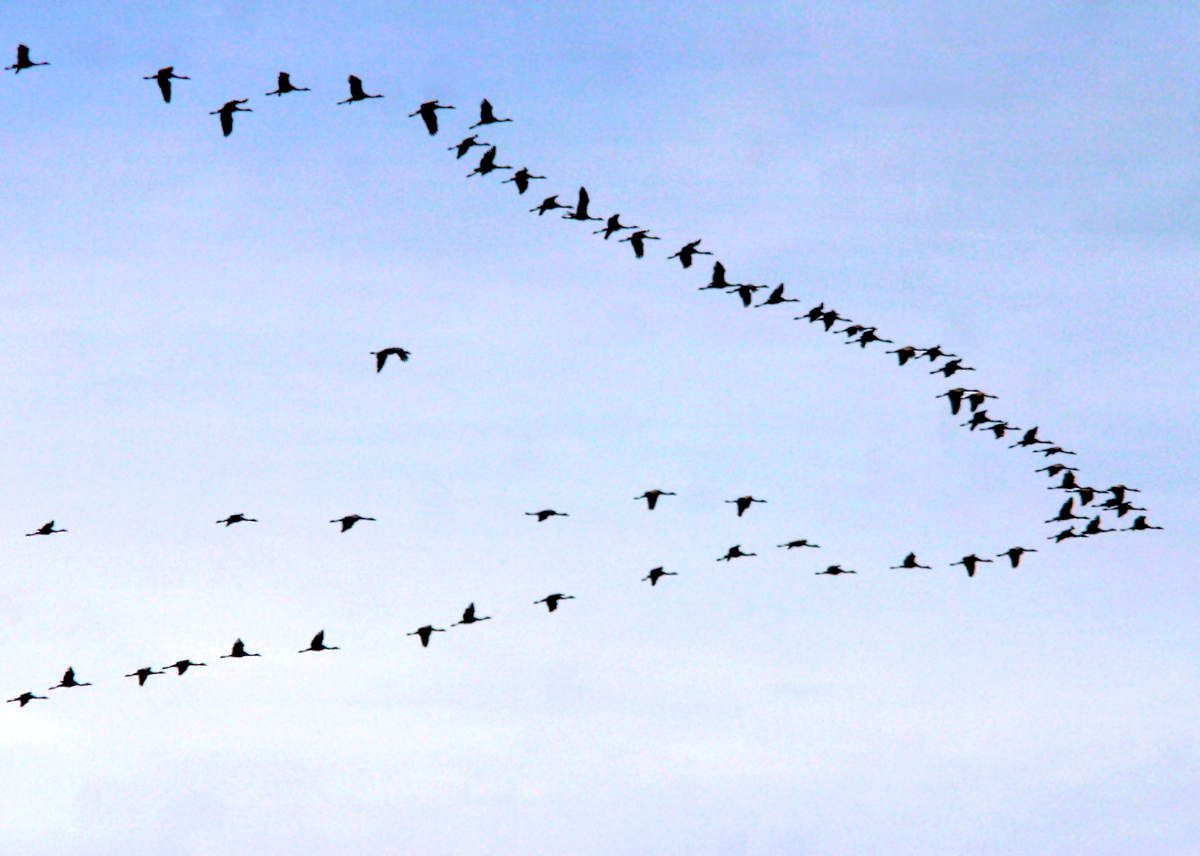
\includegraphics[width=6cm]{images/grues.jpg} \\ Migration des grues \end{center}}
			\end{column}
			
			\begin{column}{0.5\paperwidth}
				\begin{itemize}
					\item<1-> Tamás \textsc{Vicsek} (74 ans)~;
					\item<2-> Création du modèle en 1995~;
					\item<3-> Etude des mouvements collectifs (systèmes auto-organisés)~;
					\item<4-> Auncun agent leader dans le modèle.
				\end{itemize}			
			\end{column}
		\end{columns}		
	\end{frame}
	
\subsection{Explications sur le modèle}

\begin{frame}{Les bases du modèle}

\only<1>{\begin{center}Le modèle de \textsc{Vicsek} permet d'étudier un groupe d'agents qui se déplace dans un espace.\end{center}}
\only<1>{\begin{center} 
\includegraphics[width=4cm]{images/regle.jpg}  \end{center}}

\only<2>{\begin{center}Chacun des agents a une vitesse donnée (~en norme et en direction~) et va interagir avec ses voisins.\end{center}}
\only<2>{\begin{center} 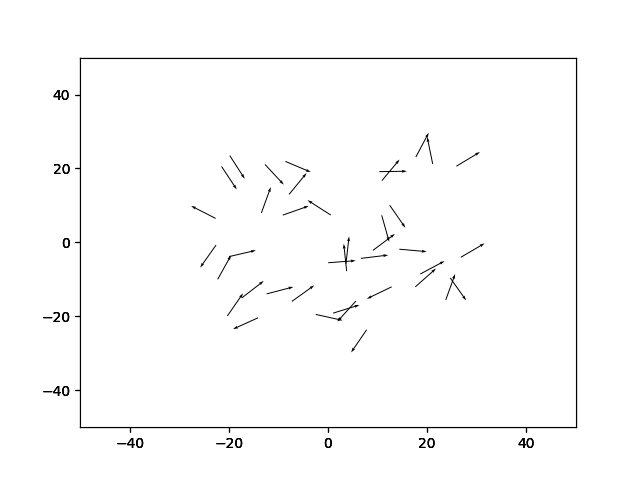
\includegraphics[width=8cm]{images/image_3.png}  \end{center}}

\only<3>{\begin{center}Création d'un mouvement de groupe suite aux interactions entre les agents.\end{center}}
\only<3>{\begin{center} 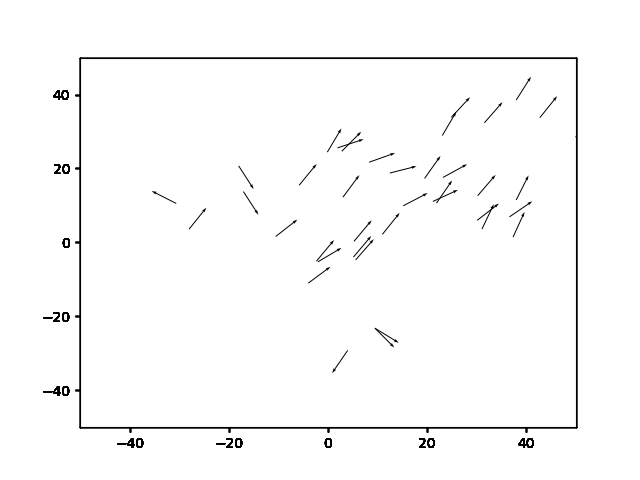
\includegraphics[width=8cm]{images/image_4.png}  \end{center}}

\end{frame}

\begin{frame}{Les équations du modèle}

		\only<1-3>{\begin{center} \[ \left\{ \begin{array}{rcl}
		r_{i}(t + \text dt) & = & r_{i}(t) + v_{i}\Delta t \\
		\Theta_{i}(t + \text dt) & = & \Theta_{j |r_{i}-r_{j}|<r} + \eta_{i}(t) \\
	\end{array} \right. \]  \end{center}} 
		\begin{itemize}
				   \item<1-3> $r_{i}$ la position de chaque individu, $v_i$ la vitesse~;
				   \item<2-3> $i$ est l'indice de l'agent en question et $t$ le temps~;
				   \item<3-3> $\eta$ le bruit et $\Theta$ l'angle définissant la direction de sa vitesse.
		\end{itemize}
				
		\vspace{-2cm}\only<4-5>{\begin{center} \[ \left\{ \begin{array}{rcl}
		r_{i}(t + \text dt) & = & r_{i}(t) + v_{i}\Delta t \\
		\Theta_{i}(t + \text dt) & = & \Theta_{j |r_{i}-r_{j}|<r} + \eta_{i}(t)
	\end{array} \right. \]  \end{center}} 
		\begin{itemize}
				   \item<4-> $\Theta_{j |r_{i}-r_{j}|<r}$ est la direction moyenne des vitesses des agents dans un cercle de rayon $r$~;
					\item<5->  $j$ représentera alors l'ensemble des voisins de $i$ compris dans ce cercle.		
					
		\end{itemize}
	\end{frame}
	
\begin{frame}{Autres intérêts du modèle}
\only<1>{\begin{center}Comportement des foules et construction de bâtiments\end{center}}
\only<1>{\begin{center} 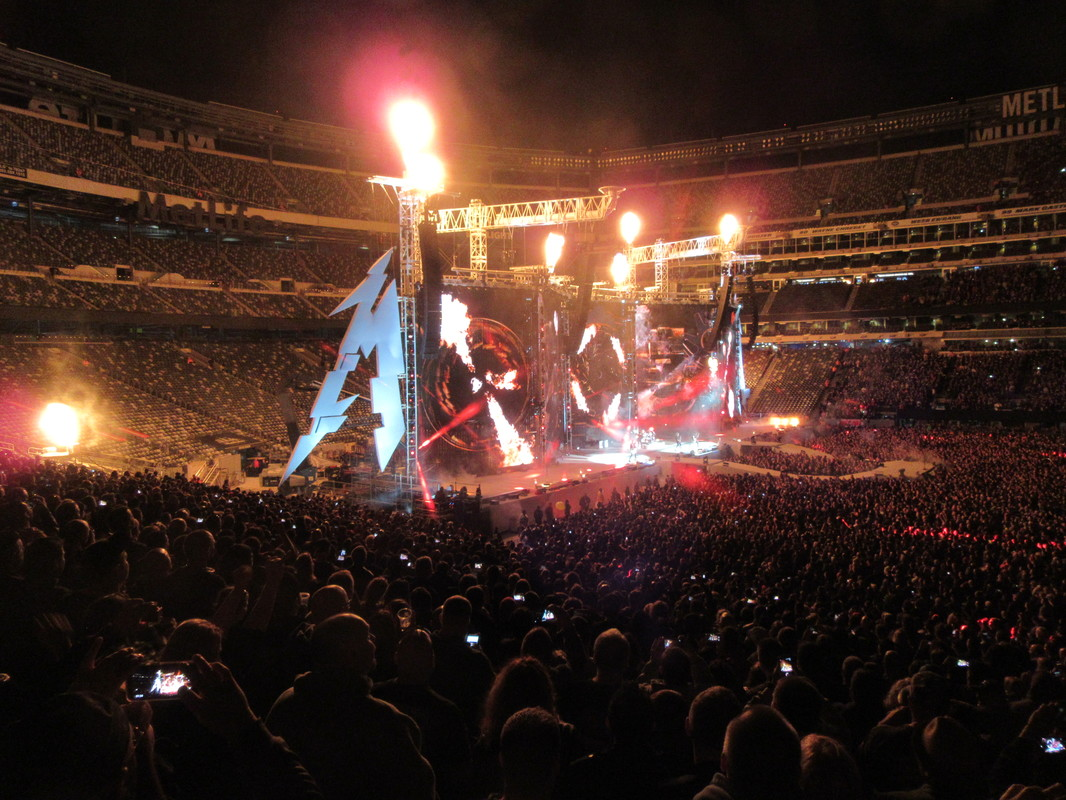
\includegraphics[width=8cm]{images/foule.jpg}  \end{center}}

\only<2>{\begin{center} Domaine de la robotique\end{center}}
\only<2>{\begin{center} 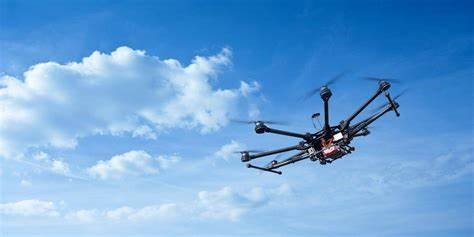
\includegraphics[width=8cm]{images/drone.jpg}  \end{center}}

\end{frame}

\section{Méthode utilisée}
\subsection{Classes et méthodes}
\begin{frame}{Classes et méthodes}
\only<1>{\begin{center} Programmation orientée objet $\Rightarrow$ Deux classes composées de  plusieurs méthodes\end{center}}
\only<1>{\begin{center} 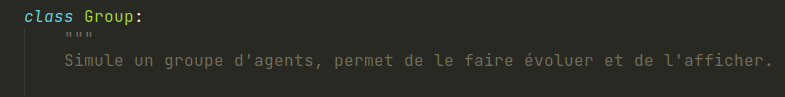
\includegraphics[width=10cm]{images/code.png} \\ 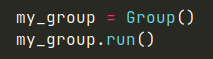
\includegraphics[width=5cm]{images/code2.png} \end{center}}
\end{frame}

\subsection{Créations et manipulations sur les agents}
\begin{frame}{Création et manipulation d'agents}
\begin{itemize}
\item Créations d'agents~;
\item Choix des paramètres (bruit, vitesse, cône de vision $\dots$)~;
\item Evolution dans le temps grâce aux équations.
\end{itemize}
\vspace{1cm}
\begin{center}$r_{i}(t + \text dt)  =  r_{i}(t) + v_{i}\Delta t$\end{center}
\end{frame}

\begin{frame}{Création et manipulation de groupe}
\begin{itemize}
\item Création de groupes~;
\item Evolution dans le temps en fonction des voisins~;
\item Calcul du paramètre d'alignement.
\end{itemize}
\vspace{1cm}
\begin{center}$\Theta_{i}(t + \text dt)  =  \Theta_{j |r_{i}-r_{j}|<r} + \eta_{i}(t)$\end{center}
\end{frame}

\section{Résultats et interprétations physiques}
\subsection{Premiers résultats et paramètres importants}

\begin{frame}{Mouvements de groupe}

\only<1>{\begin{center} 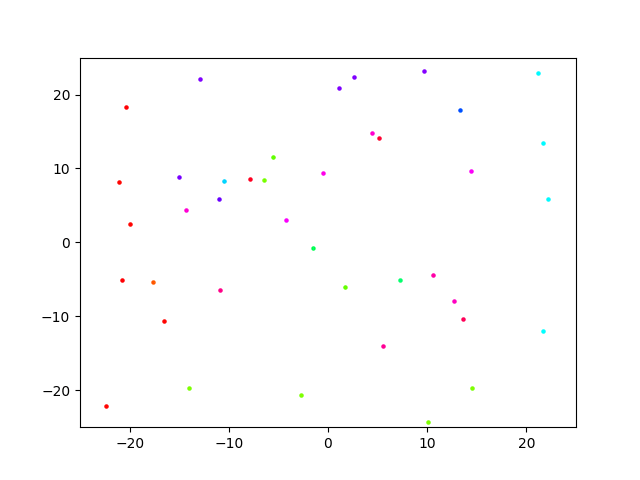
\includegraphics[width=8cm]{images/image_8.png}  \end{center}}
\only<1>{\begin{center}Images avec agents colorés pour indiquer leur direction\end{center}}


\transduration<2-50>{0.01}
	\only<2>{\begin{center} 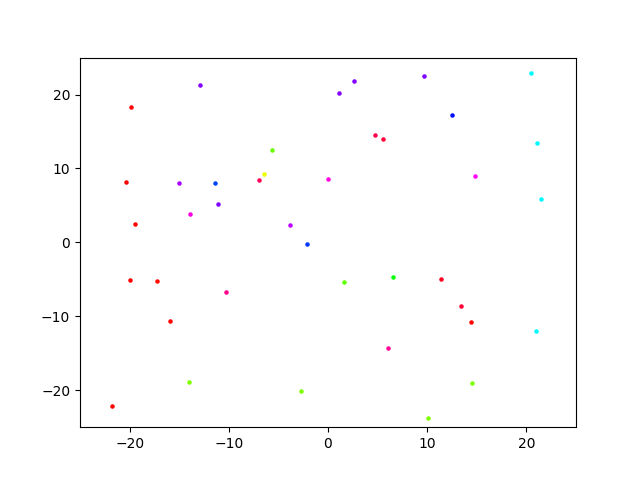
\includegraphics[width=8cm]{images/anim/01.png} \end{center}}
	\only<3>{\begin{center} 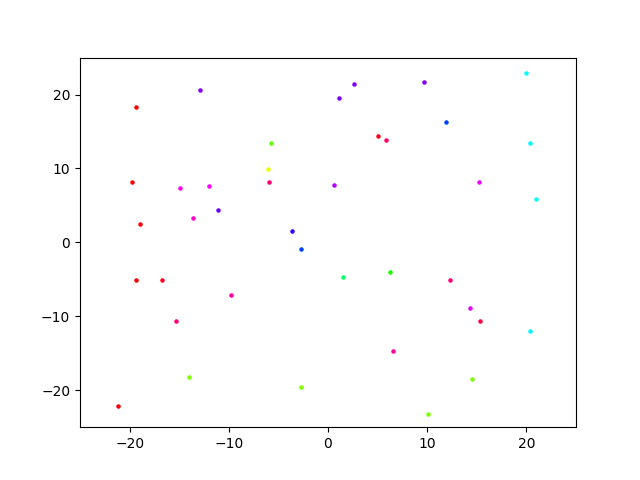
\includegraphics[width=8cm]{images/anim/02.png} \end{center}}
	\only<4>{\begin{center} 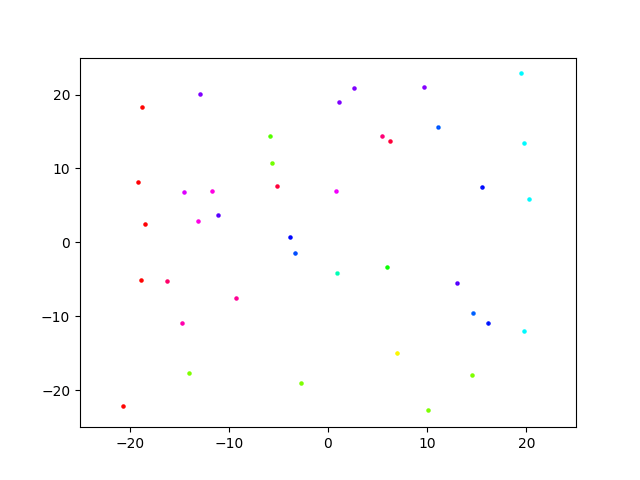
\includegraphics[width=8cm]{images/anim/03.png} \end{center}}
	\only<5>{\begin{center} 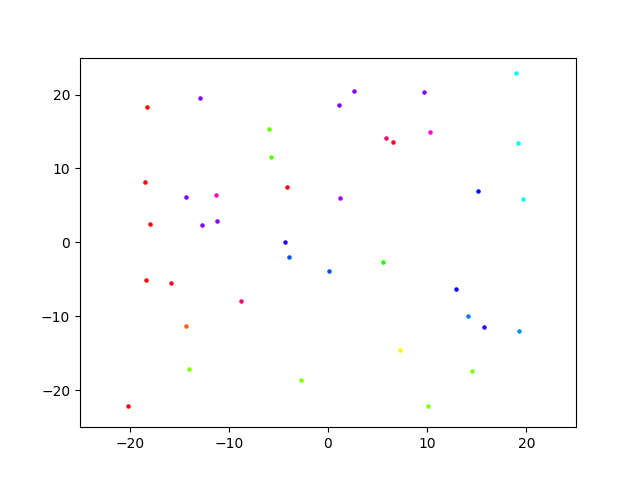
\includegraphics[width=8cm]{images/anim/04.png} \end{center}}
	\only<6>{\begin{center} 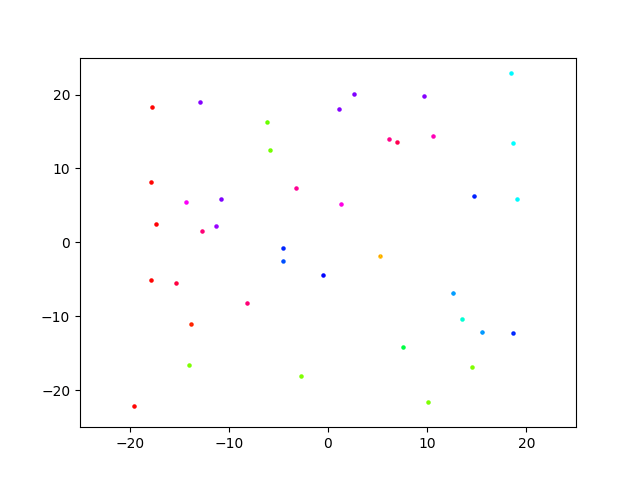
\includegraphics[width=8cm]{images/anim/05.png} \end{center}}
	\only<7>{\begin{center} 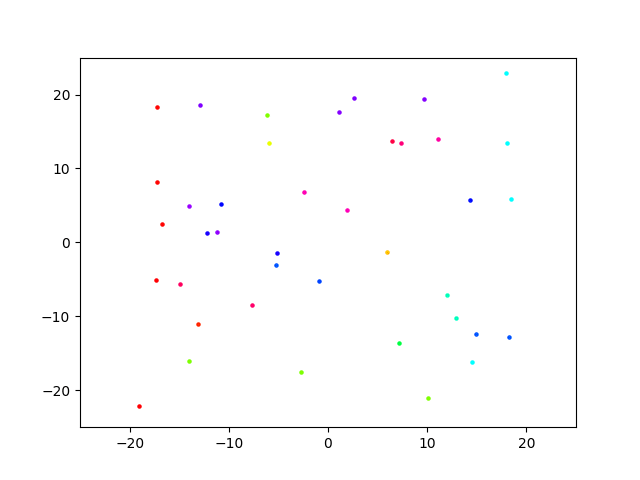
\includegraphics[width=8cm]{images/anim/06.png} \end{center}}
	\only<8>{\begin{center} 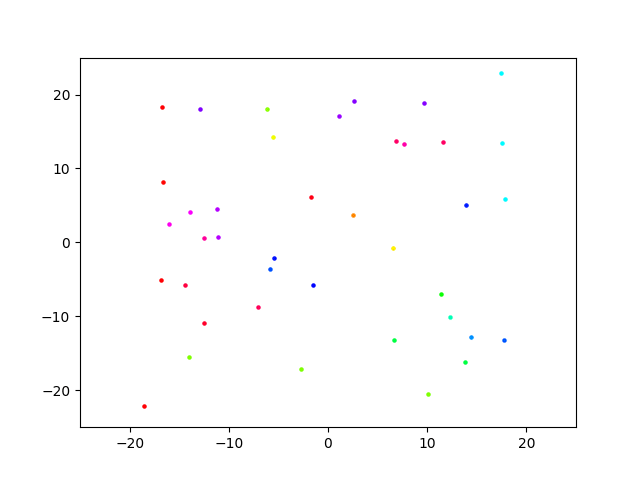
\includegraphics[width=8cm]{images/anim/07.png} \end{center}}
	\only<9>{\begin{center} 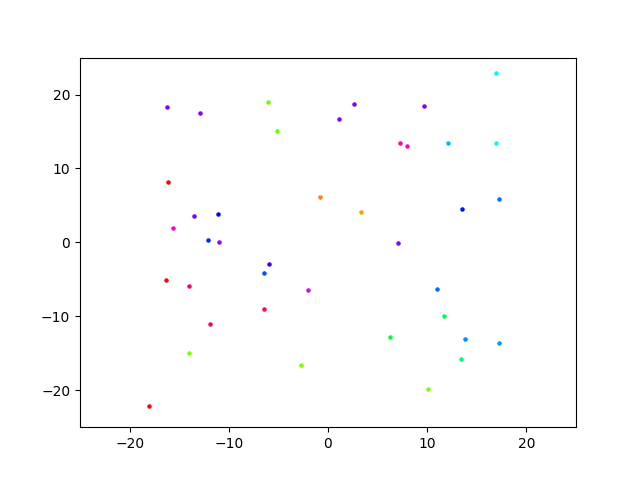
\includegraphics[width=8cm]{images/anim/08.png} \end{center}}
	\only<10>{\begin{center} 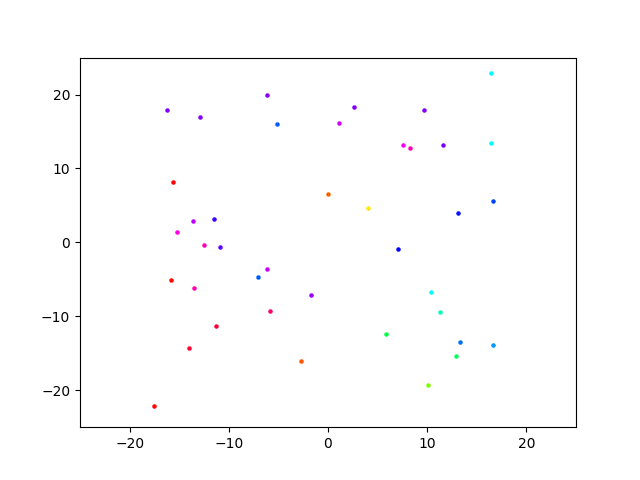
\includegraphics[width=8cm]{images/anim/09.png} \end{center}}
	\only<11>{\begin{center} 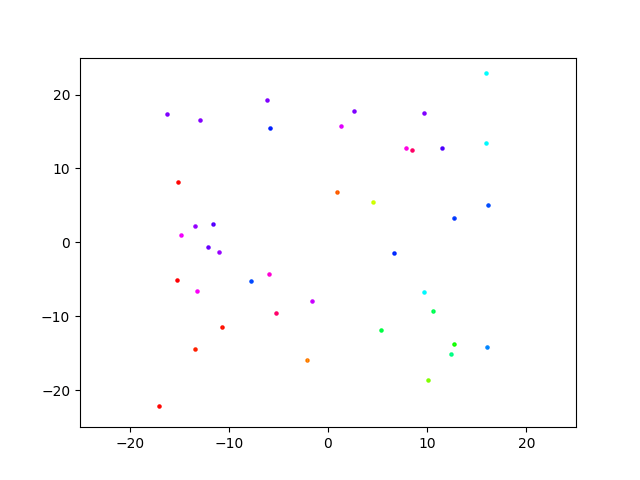
\includegraphics[width=8cm]{images/anim/10.png} \end{center}}
	\only<12>{\begin{center} 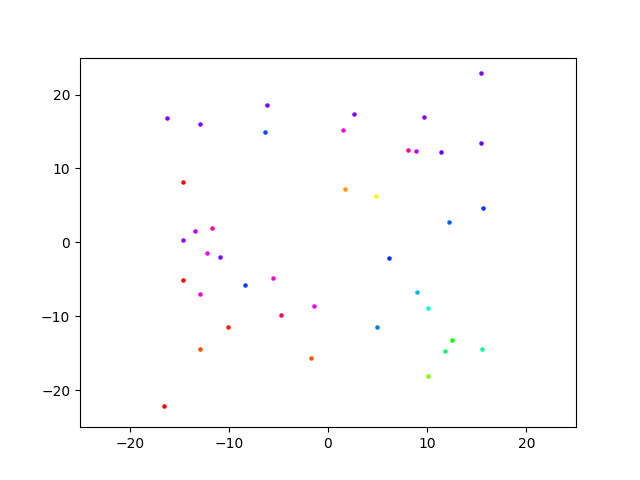
\includegraphics[width=8cm]{images/anim/11.png} \end{center}}
	\only<13>{\begin{center} 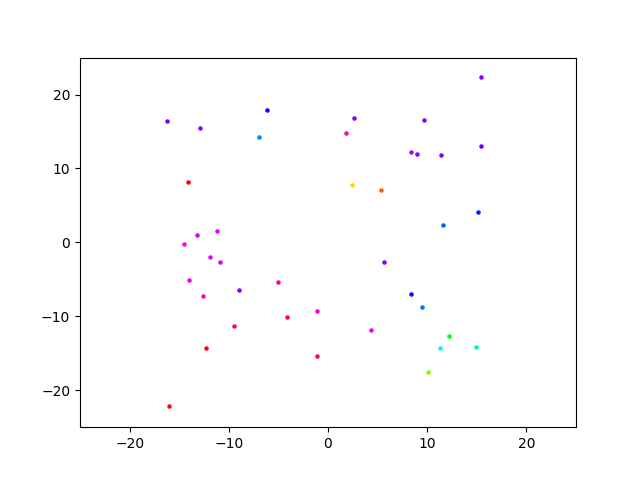
\includegraphics[width=8cm]{images/anim/12.png} \end{center}}
	\only<14>{\begin{center} 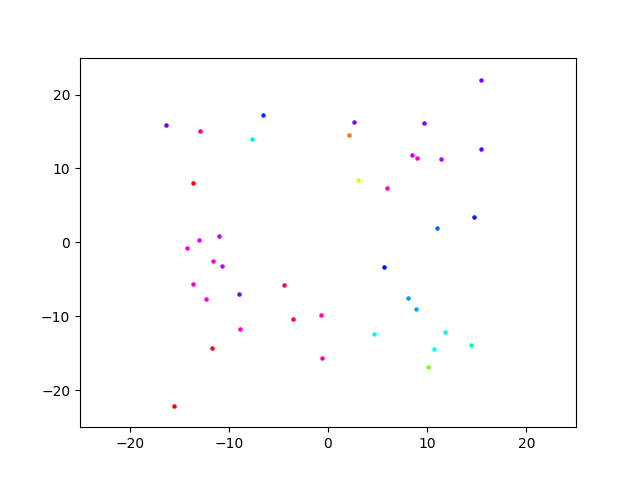
\includegraphics[width=8cm]{images/anim/13.png} \end{center}}
	\only<15>{\begin{center} 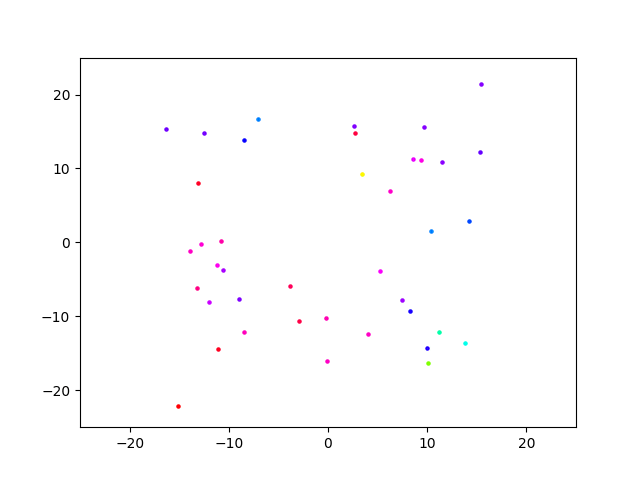
\includegraphics[width=8cm]{images/anim/14.png} \end{center}}
	\only<16>{\begin{center} 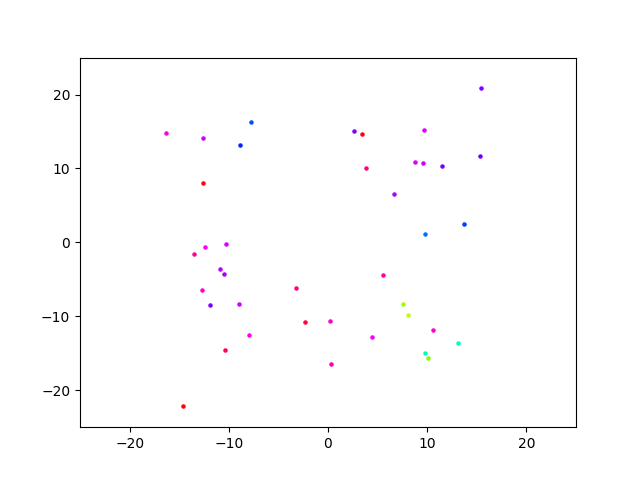
\includegraphics[width=8cm]{images/anim/15.png} \end{center}}
	\only<17>{\begin{center} 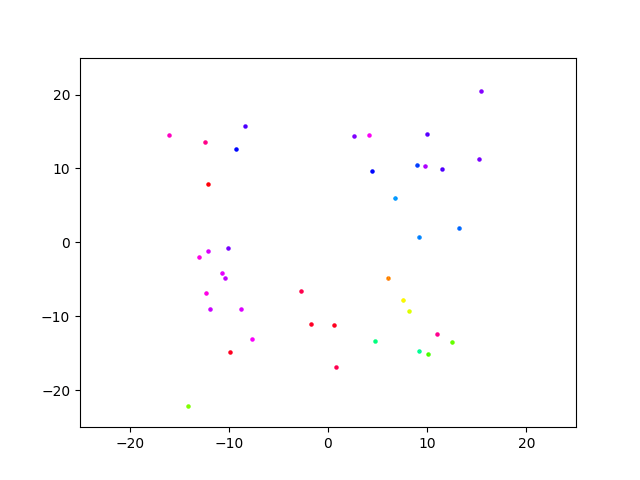
\includegraphics[width=8cm]{images/anim/16.png} \end{center}}
	\only<18>{\begin{center} 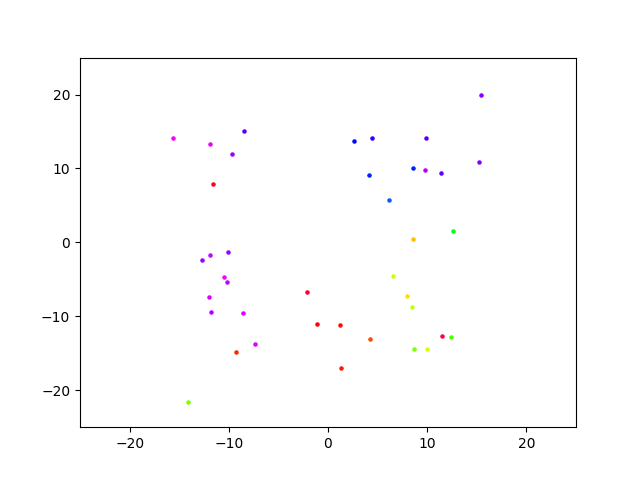
\includegraphics[width=8cm]{images/anim/17.png} \end{center}}
	\only<19>{\begin{center} 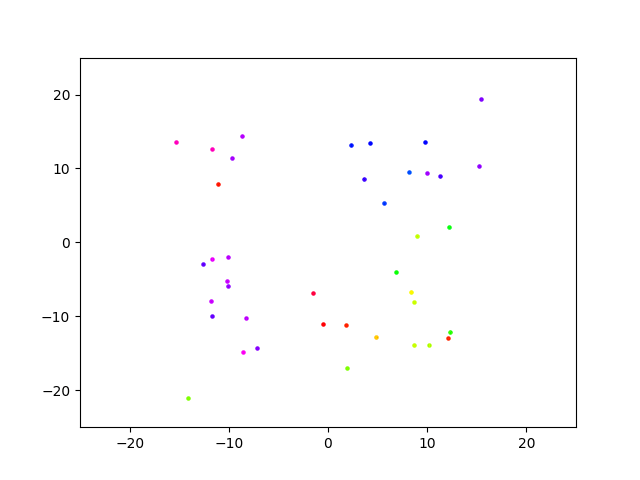
\includegraphics[width=8cm]{images/anim/18.png} \end{center}}
	\only<20>{\begin{center} 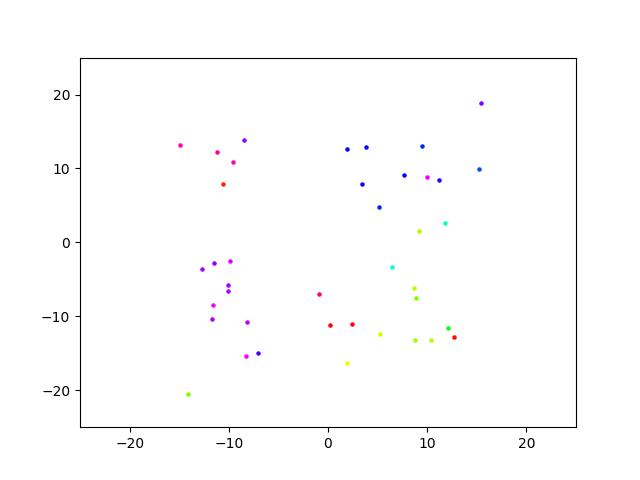
\includegraphics[width=8cm]{images/anim/19.png} \end{center}}
	\only<21>{\begin{center} 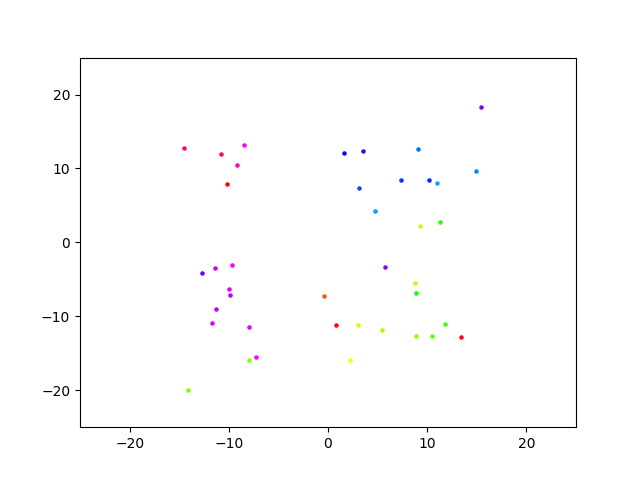
\includegraphics[width=8cm]{images/anim/20.png} \end{center}}
	\only<22>{\begin{center} 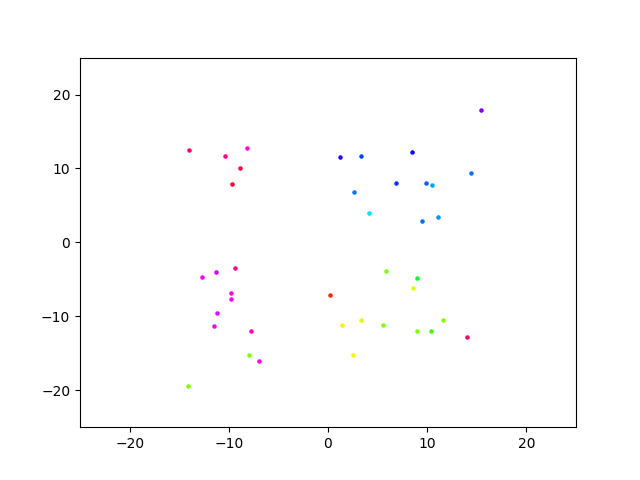
\includegraphics[width=8cm]{images/anim/21.png} \end{center}}
	\only<23>{\begin{center} 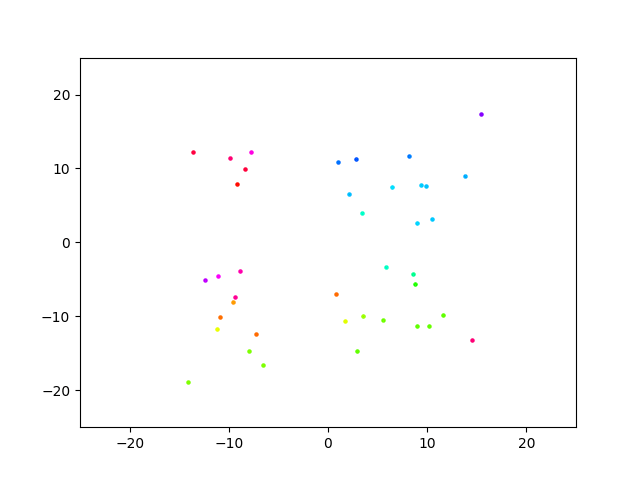
\includegraphics[width=8cm]{images/anim/22.png} \end{center}}
	\only<24>{\begin{center} 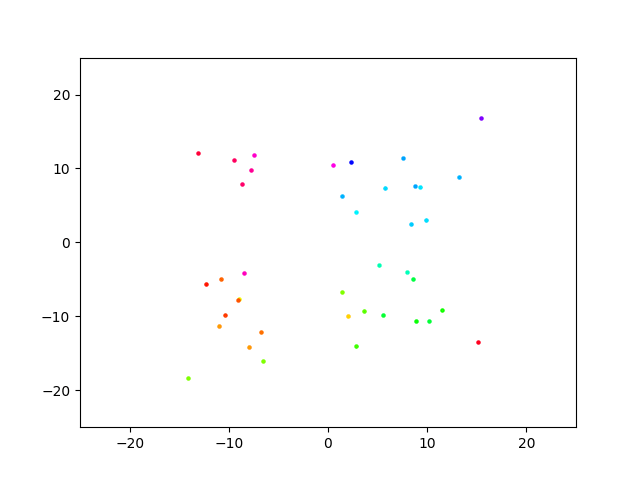
\includegraphics[width=8cm]{images/anim/23.png} \end{center}}
	\only<25>{\begin{center} 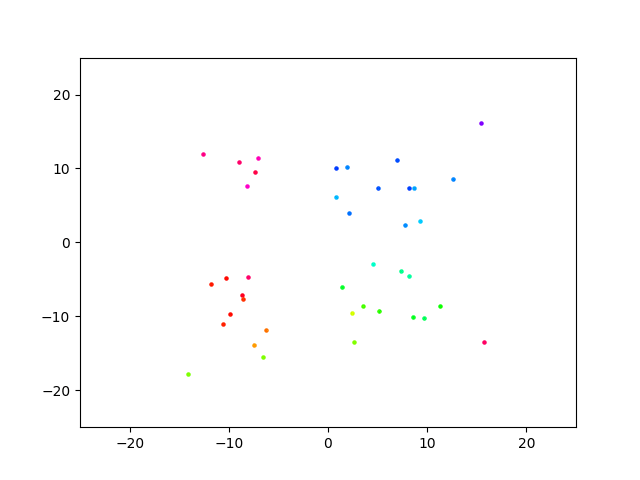
\includegraphics[width=8cm]{images/anim/24.png} \end{center}}
	\only<26>{\begin{center} 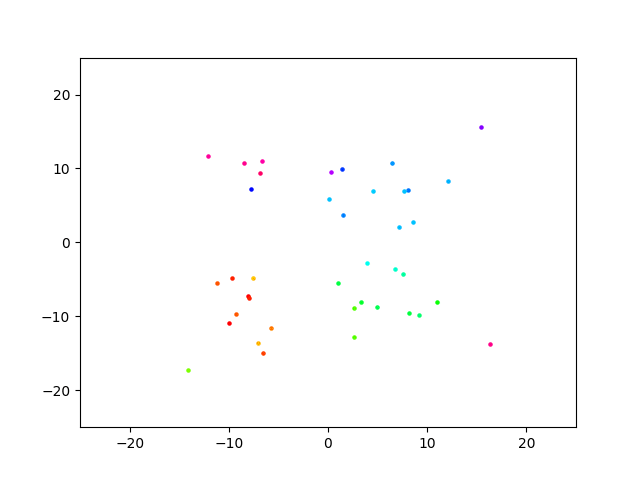
\includegraphics[width=8cm]{images/anim/25.png} \end{center}}
	\only<27>{\begin{center} 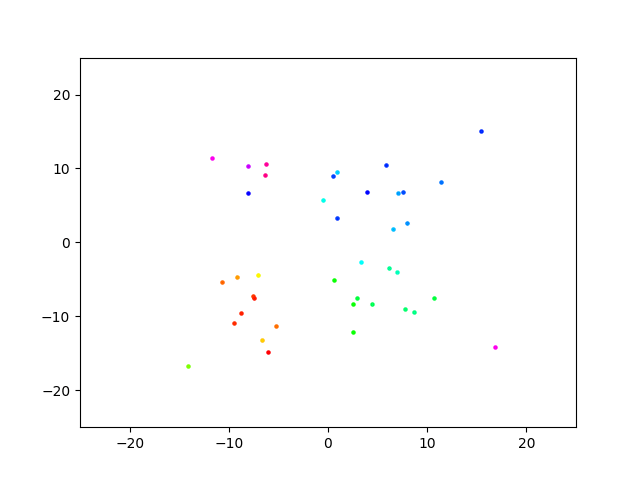
\includegraphics[width=8cm]{images/anim/26.png} \end{center}}
	\only<28>{\begin{center} 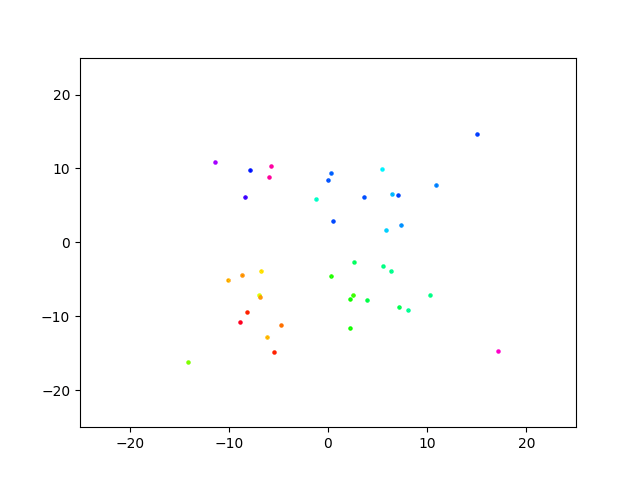
\includegraphics[width=8cm]{images/anim/27.png} \end{center}}
	\only<29>{\begin{center} 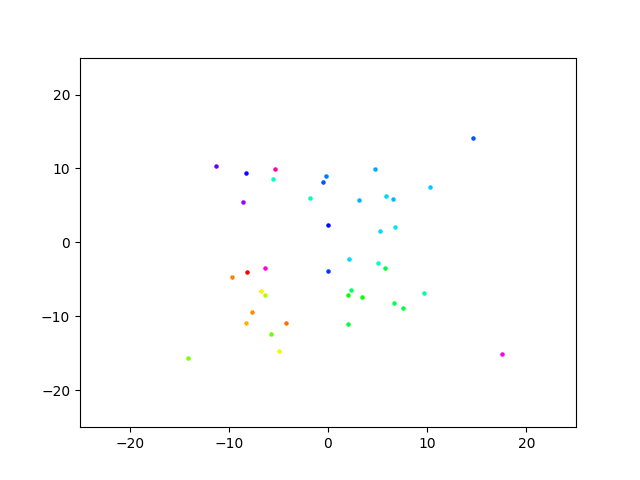
\includegraphics[width=8cm]{images/anim/28.png} \end{center}}
	\only<30>{\begin{center} 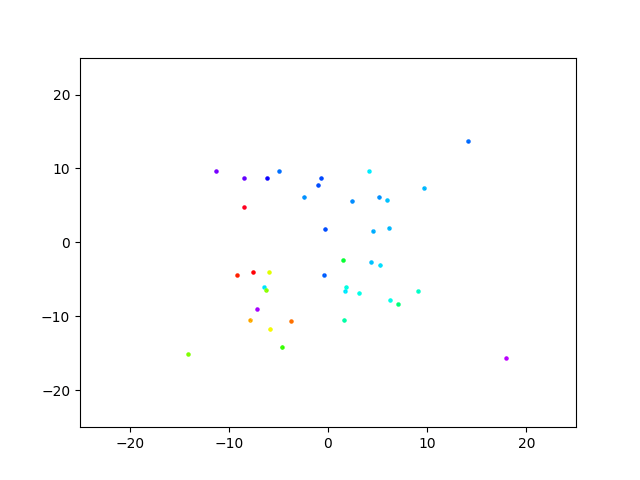
\includegraphics[width=8cm]{images/anim/29.png} \end{center}}
	\only<31>{\begin{center} 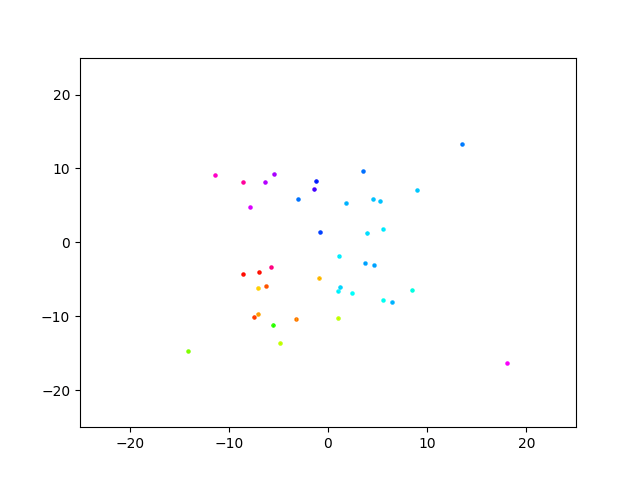
\includegraphics[width=8cm]{images/anim/30.png} \end{center}}
	\only<32>{\begin{center} 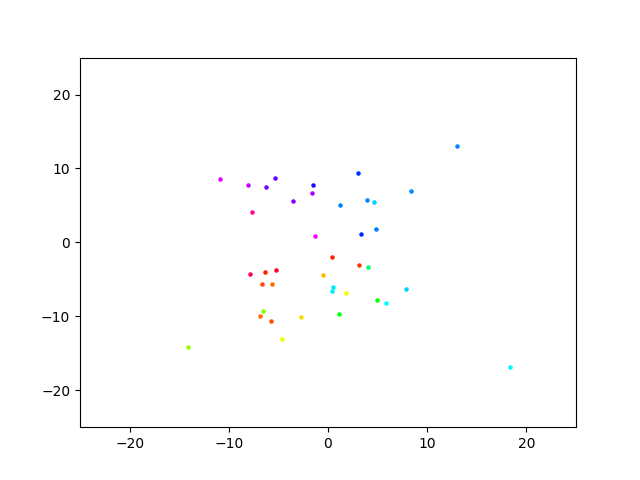
\includegraphics[width=8cm]{images/anim/31.png} \end{center}}
	\only<33>{\begin{center} 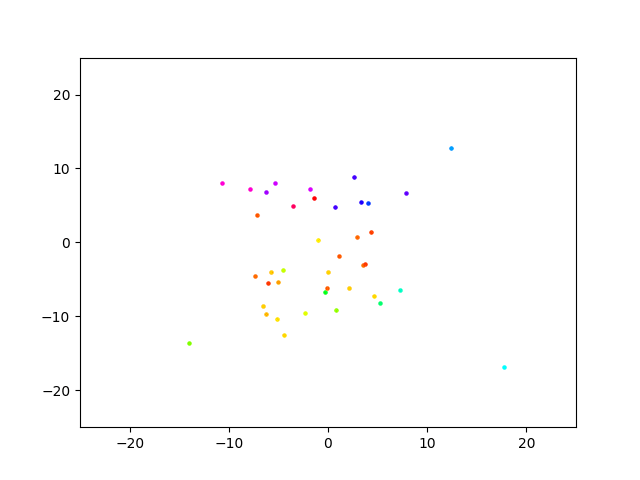
\includegraphics[width=8cm]{images/anim/32.png} \end{center}}
	\only<34>{\begin{center} 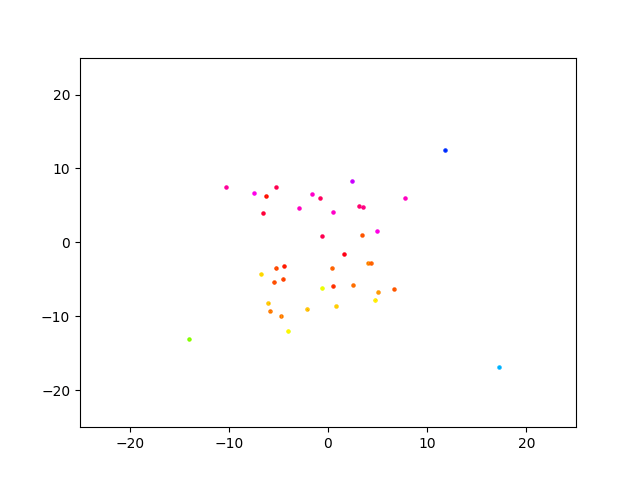
\includegraphics[width=8cm]{images/anim/33.png} \end{center}}
	\only<35>{\begin{center} 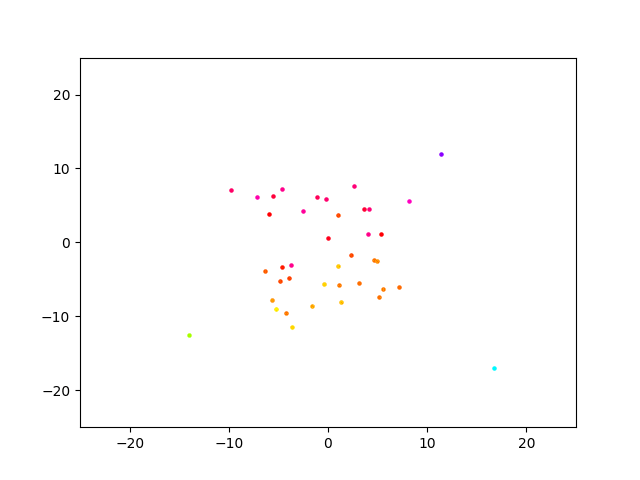
\includegraphics[width=8cm]{images/anim/34.png} \end{center}}
	\only<36>{\begin{center} 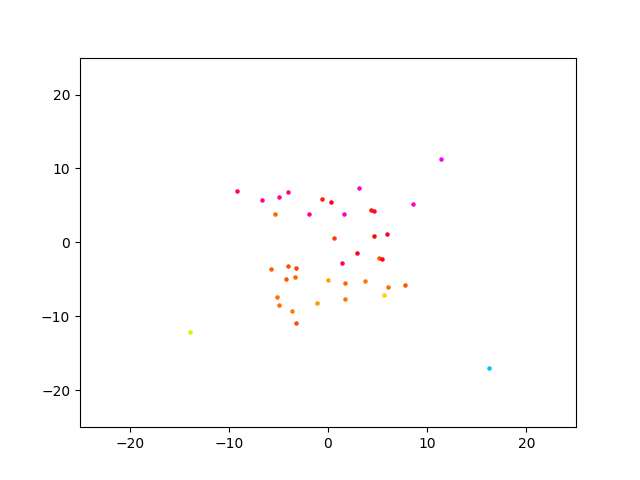
\includegraphics[width=8cm]{images/anim/35.png} \end{center}}
	\only<37>{\begin{center} 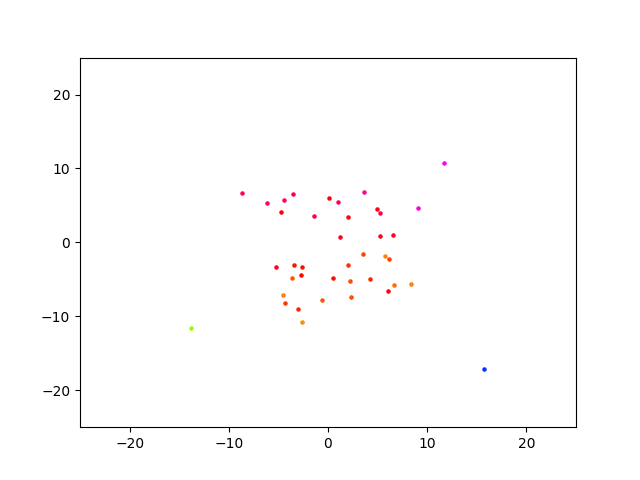
\includegraphics[width=8cm]{images/anim/36.png} \end{center}}
	\only<38>{\begin{center} \includegraphics[width=8cm]{images/anim/37.png} \end{center}}
	\only<39>{\begin{center} \includegraphics[width=8cm]{images/anim/38.png} \end{center}}
	\only<40>{\begin{center} \includegraphics[width=8cm]{images/anim/39.png} \end{center}}
	\only<41>{\begin{center} \includegraphics[width=8cm]{images/anim/40.png} \end{center}}
	\only<42>{\begin{center} \includegraphics[width=8cm]{images/anim/41.png} \end{center}}
	\only<43>{\begin{center} \includegraphics[width=8cm]{images/anim/42.png} \end{center}}
	\only<44>{\begin{center} \includegraphics[width=8cm]{images/anim/43.png} \end{center}}
	\only<45>{\begin{center} \includegraphics[width=8cm]{images/anim/44.png} \end{center}}
	\only<46>{\begin{center} \includegraphics[width=8cm]{images/anim/45.png} \end{center}}
	\only<47>{\begin{center} \includegraphics[width=8cm]{images/anim/46.png} \end{center}}
	\only<48>{\begin{center} \includegraphics[width=8cm]{images/anim/47.png} \end{center}}
	\only<49>{\begin{center} \includegraphics[width=8cm]{images/anim/48.png} \end{center}}
	\only<50>{\begin{center} \includegraphics[width=8cm]{images/anim/49.png} \end{center}}
	
	\only<51>{\begin{center} \includegraphics[width=8cm]{images/anim/49.png} \end{center}}

\end{frame}



\begin{frame}{Cône de vision}
\begin{columns}
			\begin{column}{0.6\paperwidth}
		       \begin{center}\includegraphics[width=8cm]{images/image_12.png}\end{center}
			\end{column}
			
			\begin{column}{0.4\paperwidth}
				\begin{itemize}
					\item<1-> Meilleure visualisation des voisins visibles par l'agent~;
					\item<2-> Images trop chargées pour observer correctement les mouvements de groupe.
				\end{itemize}			
			\end{column}
		\end{columns}		
	\end{frame}

\begin{frame}{Paramètre de bruit}
\begin{columns}
			\begin{column}{0.6\paperwidth}
		       	\transduration<1-49>{0.01}
				\only<1>{\begin{center} \includegraphics[width=8cm]{images/bruit/01.png} \end{center}}
				\only<2>{\begin{center} \includegraphics[width=8cm]{images/bruit/02.png} \end{center}}
				\only<3>{\begin{center} \includegraphics[width=8cm]{images/bruit/03.png} \end{center}}
				\only<4>{\begin{center} \includegraphics[width=8cm]{images/bruit/04.png} \end{center}}
				\only<5>{\begin{center} \includegraphics[width=8cm]{images/bruit/05.png} \end{center}}
				\only<6>{\begin{center} \includegraphics[width=8cm]{images/bruit/06.png} \end{center}}
				\only<7>{\begin{center} \includegraphics[width=8cm]{images/bruit/07.png} \end{center}}
				\only<8>{\begin{center} \includegraphics[width=8cm]{images/bruit/08.png} \end{center}}
				\only<9>{\begin{center} \includegraphics[width=8cm]{images/bruit/09.png} \end{center}}
				\only<10>{\begin{center} \includegraphics[width=8cm]{images/bruit/10.png} \end{center}}
				\only<11>{\begin{center} \includegraphics[width=8cm]{images/bruit/11.png} \end{center}}
				\only<12>{\begin{center} \includegraphics[width=8cm]{images/bruit/12.png} \end{center}}
				\only<13>{\begin{center} \includegraphics[width=8cm]{images/bruit/13.png} \end{center}}
				\only<14>{\begin{center} \includegraphics[width=8cm]{images/bruit/14.png} \end{center}}
				\only<15>{\begin{center} \includegraphics[width=8cm]{images/bruit/15.png} \end{center}}
				\only<16>{\begin{center} \includegraphics[width=8cm]{images/bruit/16.png} \end{center}}
				\only<17>{\begin{center} \includegraphics[width=8cm]{images/bruit/17.png} \end{center}}
				\only<18>{\begin{center} \includegraphics[width=8cm]{images/bruit/18.png} \end{center}}
				\only<19>{\begin{center} \includegraphics[width=8cm]{images/bruit/19.png} \end{center}}
				\only<20>{\begin{center} \includegraphics[width=8cm]{images/bruit/20.png} \end{center}}
				\only<21>{\begin{center} \includegraphics[width=8cm]{images/bruit/21.png} \end{center}}
				\only<22>{\begin{center} \includegraphics[width=8cm]{images/bruit/22.png} \end{center}}
				\only<23>{\begin{center} \includegraphics[width=8cm]{images/bruit/23.png} \end{center}}
				\only<24>{\begin{center} \includegraphics[width=8cm]{images/bruit/24.png} \end{center}}
				\only<25>{\begin{center} \includegraphics[width=8cm]{images/bruit/25.png} \end{center}}
				\only<26>{\begin{center} \includegraphics[width=8cm]{images/bruit/26.png} \end{center}}
				\only<27>{\begin{center} \includegraphics[width=8cm]{images/bruit/27.png} \end{center}}
				\only<28>{\begin{center} \includegraphics[width=8cm]{images/bruit/28.png} \end{center}}
				\only<29>{\begin{center} \includegraphics[width=8cm]{images/bruit/29.png} \end{center}}
				\only<30>{\begin{center} \includegraphics[width=8cm]{images/bruit/30.png} \end{center}}
				\only<31>{\begin{center} \includegraphics[width=8cm]{images/bruit/31.png} \end{center}}
				\only<32>{\begin{center} \includegraphics[width=8cm]{images/bruit/32.png} \end{center}}
				\only<33>{\begin{center} \includegraphics[width=8cm]{images/bruit/33.png} \end{center}}
				\only<34>{\begin{center} \includegraphics[width=8cm]{images/bruit/34.png} \end{center}}
				\only<35>{\begin{center} \includegraphics[width=8cm]{images/bruit/35.png} \end{center}}
				\only<36>{\begin{center} \includegraphics[width=8cm]{images/bruit/36.png} \end{center}}
				\only<37>{\begin{center} \includegraphics[width=8cm]{images/bruit/37.png} \end{center}}
				\only<38>{\begin{center} \includegraphics[width=8cm]{images/bruit/38.png} \end{center}}
				\only<39>{\begin{center} \includegraphics[width=8cm]{images/bruit/39.png} \end{center}}
				\only<40>{\begin{center} \includegraphics[width=8cm]{images/bruit/40.png} \end{center}}
				\only<41>{\begin{center} \includegraphics[width=8cm]{images/bruit/41.png} \end{center}}
				\only<42>{\begin{center} \includegraphics[width=8cm]{images/bruit/42.png} \end{center}}
				\only<43>{\begin{center} \includegraphics[width=8cm]{images/bruit/43.png} \end{center}}
				\only<44>{\begin{center} \includegraphics[width=8cm]{images/bruit/44.png} \end{center}}
				\only<45>{\begin{center} \includegraphics[width=8cm]{images/bruit/45.png} \end{center}}
				\only<46>{\begin{center} \includegraphics[width=8cm]{images/bruit/46.png} \end{center}}
				\only<47>{\begin{center} \includegraphics[width=8cm]{images/bruit/47.png} \end{center}}
				\only<48>{\begin{center} \includegraphics[width=8cm]{images/bruit/48.png} \end{center}}
				\only<49>{\begin{center} \includegraphics[width=8cm]{images/bruit/49.png} \end{center}}
				\only<50>{\begin{center} \includegraphics[width=8cm]{images/bruit/50.png} \end{center}}
			\end{column}
			
			\begin{column}{0.4\paperwidth}
				\begin{itemize}
					\item<1-> Ce paramètre perturbe la communication entre les agents~;
					\item<50-> La cohésion du groupe est significativement réduite lorsque le bruit augmente.
          \end{itemize}			
			\end{column}
		\end{columns}		
	\end{frame}

\subsection{Résultats historiques de Vicsek}

\begin{frame}{Paramètre d'alignement en fonction du bruit}
   \only<1>{\begin{center}\includegraphics[width=8cm]{images/bruit_4bis.png}\end{center}}
   \only<1>{\begin{center} 40 agents \\ Densité fixe $\rightarrow$ 4,15 agents par unité de surface\end{center}}

   \only<2>{
	\begin{columns}
	\begin{column}{0.5\paperwidth}
   		\begin{center}\includegraphics[width=6cm]{images/comparatif_4.png}\end{center}
	\end{column}
	\begin{column}{0.5\paperwidth}
		\begin{center} \includegraphics[width=6cm]{images/bruit_vicsek.png} \end{center}
	\end{column}
	\end{columns}
	}
   \only<2>{\begin{center}À bruit égal, augmenter le nombre d'agent $\Rightarrow$ alignement dégradé \end{center}}
\end{frame}

\begin{frame}{Paramètre d'alignement en fonction de la densité}
	\begin{columns}
	\begin{column}{0.5\paperwidth}
 		\begin{center}\includegraphics[width=6cm]{images/densite_1[noise=1]2.png}\end{center}
   	\end{column}
	\begin{column}{0.5\paperwidth}
 		\begin{center}\includegraphics[width=6cm]{images/densite_vicsek.png}\end{center}
   	\end{column}
	\end{columns}

	\begin{center} Bruit fixé à 1 \\ Densité plus forte $\rightarrow$ Meilleur alignement \end{center}
\end{frame}

\subsection{Au-delà du modèle de Vicsek}
\begin{frame}{Création d'un agent leader}
		\begin{columns}
			\begin{column}{0.6\paperwidth}
			\only<1-3>{\begin{center} \includegraphics[width=7.5cm]{images/image_15.png} \\ Un agent leader en noir \end{center}}
			\only<4>{\begin{center} \includegraphics[width=6cm]{images/grues.jpg} \\ Migration des grues \end{center}}
			\end{column}
			
			\begin{column}{0.4\paperwidth}
				\begin{itemize}
					\item<1-> Nouveau paramètre pour le type d'agent~;
					\item<2-> Influence plus importante sur les agents normaux~;
					\item<3-> Organisation en «~triangle ou en arc de cercle~»~;
					\item<4-> Autre type de mouvement collectif.
				\end{itemize}			
			\end{column}
		\end{columns}		
	\end{frame}
	
\begin{frame}{Mise en place d'une prédation}	
\begin{columns}
			\begin{column}{0.6\paperwidth}
			\only<1-3>{\begin{center} \includegraphics[width=7.5cm]{images/image_16.png} \\Trois prédateurs en noir \end{center}}
			\only<4>{\begin{center} \includegraphics[width=7.5cm]{images/image_17.png} \\Un seul prédateur en noir \end{center}}
			\end{column}
			
			\begin{column}{0.4\paperwidth}
				\begin{itemize}
					\item<1-> Nouveau paramètre pour simuler la «~peur des agents~»~;
					\item<2-> Agents prennent la fuite dans le sens inverse de leur direction~;
					\item<3-> Mouvements de groupes moins observés avec plusieurs prédateurs~;
					\item<4-> Mouvements de groupes conservés avec un prédateur.
				\end{itemize}			
			\end{column}
		\end{columns}		
	\end{frame}

\begin{frame}{Système évolutif}	

\begin{center}Nous avons 4 groupes tests avec des paramètres différents.\end{center}

\begin{center}\begin{tabular}{|c|c|c|} \hline	
          \centering	
			bruit & sensibilité & pourcentage de survivants \\ \hline
			0 & 0 & 39 \\ \hline
			0 & 1 & 79 \\ \hline
			1 & 0 & 30 \\ \hline
			1 & 1 & 86 \\ \hline
		\end{tabular}\end{center}
		
\begin{center}Bruit et sensibilité au maximum $\rightarrow$ Meilleure chance de survie.\end{center}
\end{frame}

\begin{frame}{Ajout d'obstacles}
\only<1>{\begin{center} \includegraphics[width=7.5cm]{images/image_19.png}  \end{center}}
\only<1>{\begin{center} Nouveau type d'agent «~mur~»\end{center}}

\only<2>{\begin{center}\includegraphics[width=7.5cm]{images/image_18.png}\end{center}} 
\only<2>{\begin{center} La majorité des agents fait demi-tour \\ Importance de la taille de l'obstacle\end{center}}

\only<3>{\begin{center}\includegraphics[width=7.5cm]{images/image_20.png}\end{center}} 
\only<3>{\begin{center} Simulation de petits obstacles en noir \end{center}}

\only<4>{\begin{center}\includegraphics[width=7.5cm]{images/image_21.png}\end{center}} 
\only<4>{\begin{center} Les agents contournent les obstacles \end{center}}
\end{frame}

\section*{\ }
	\begin{frame}{Conclusion}
		
			\begin{itemize}
				\item<1-> Nous avons réussi à simuler le modèle de Vicsek numériquement~;
				\item<2-> Nous avons joué sur le fait que chaque agent est unique~;
				\item<3-> Nous sommes allés au-delà du modèle avec la mise en place d'une prédation, la création d'agents leaders et de murs.
			\end{itemize}
\end{frame}		
\begin{frame}	
\begin{center} \includegraphics[width=8cm]{images/image_9.png}  \end{center}
\begin{center} Merci pour votre écoute ! \\ Avez-vous des questions ? \end{center}
\end{frame}

\end{document}
